\section{Solving Instationary Problems}

\subsection{One Step Methods}

\begin{frame}
\frametitle{Approach for Instationary Problems}
\begin{itemize}
\item Method of lines approach:
\begin{itemize}
\item Semi-discretization in space.
\item Solve large ODE problem.
\end{itemize}
\item One step methods for ODEs
\begin{itemize}
\item Diagonally implicit Runge-Kutta methods.
\item Explicit Runge-Kutta methods.
\item Includes Explicit/implicit Euler, Crank-Nicolson, fractional
step $\theta$, Alexanders S-stable methods \cite{alexander:77}, 
Shu's explicit TVD Runge-Kutta methods \cite{shu:88}\ldots
\end{itemize}
\item Multistep methods (e.g. BDF) could be implemented easily in current approach.
\item Space-time methods are not yet supported
\begin{itemize}
\item Require extension of grid function space.
\end{itemize}
\end{itemize}
\end{frame}

\begin{frame}
\frametitle{Problem and Finite Element Formulation}
Consider the following model problem:
\begin{subequations} \label{Eq:Example03}
\begin{align*}
\partial_t u -\Delta u + a u &= f &&\text{in $\Omega\times\Sigma$}, \Sigma=(t_0,t_0+T],\\
u(\cdot,t) &= g(\cdot,t) && \text{on $\Gamma_D(t)$},\\ 
-\nabla u(\cdot,t) \cdot n &= j(\cdot,t) &&\text{on $\Gamma_N(t)=\partial\Omega\setminus\Gamma_D(t)$},\\
u(\cdot,t_0) &= u_0(\cdot) && \text{at $t=t_0$}.
\end{align*}
\end{subequations}
Semi-discretization in space. Find $u_h(t)\in w_h(t) + \tilde{U}_h^k$:
\begin{equation*}
\frac{d}{dt} \underbrace{\int_\Omega u_h v \,dx}_{m(u_h,v;t)} + \underbrace{\int_\Omega \nabla u_h \cdot \nabla v
+ a u_h v - f v \, dx + \int_{\Gamma_N} jv \, ds}_{r(u_h,v;t)} = 0 \qquad \forall v \in \tilde{U}_h^k.
\end{equation*}
$r(u,v;t)$ is known residual form, except it may depend on time.

$m(u,v;t)$ is a new form but can be described by the same interface.
\end{frame}

\begin{frame}
\frametitle{Implicit Euler Method}
Subdivide time interval
\begin{equation*}
\overline{\Sigma} = \{t^{0}\} \cup (t^0,t^1] \cup \ldots \cup (t^{N-1},t^N]
\end{equation*}
with $t^0=t_0$, $t^N=t_0+T$, $t^{n-1}<t^n$ for $1\leq n\leq N$.

Set $k^n=t^{n+1}-t^n$.

Difference quotient in time. Find $u_h \in w_h(t^{n+1}) + \tilde{U}_h^k(t^{n+1})$:
\begin{equation*}
\begin{split}
\frac{1}{k^n} \bigl\{ m\left(u_h^{n+1},v;t^{n+1}\right) &- m\left(u_h^{n},v;t^{n}\right)\bigr\} \\
&\qquad + r\left(u_h^{n+1},v;t^{n+1}\right) = 0
\qquad  \forall v \in \tilde{U}_h^k(t^{n+1}).
\end{split}
\end{equation*}

Solve (non-) linear problem per time step:
\begin{equation*}
\begin{split}
m\left(u_h^{n+1},v;t^{n+1}\right) &+ k^n r\left(u_h^{n+1},v;t^{n+1}\right)\\
&\qquad \qquad - m\left(u_h^{n},v;t^{n}\right) = 0 \qquad  \forall v \in \tilde{U}_h^k(t^{n+1}).
\end{split}
\end{equation*}
\end{frame}


\begin{frame}
\frametitle{General One Step Methods I}
The general scheme reads:
\begin{enumerate}
\item $u_h^{(0)} = u_h^{n}$.
\item For $i=1,\ldots,s\in\mathbb{N}$, find $u_h^{(i)}\in w_h(t^n+d_i k^n) + \tilde{U}^k_h(t^{n+1})$:
\begin{equation*}
\begin{split}
\sum\limits_{j=0}^{s} \biggl[a_{ij} m_h&\left(u_h^{(j)},v;t^n+d_jk^n\right) \\
&\qquad + b_{ij} k^n r_h\left(u_h^{(j)}, v;t^n+d_j k^n\right) \biggr] = 0 \qquad \forall v\in \tilde{U}^k_h(t^{n+1}).
\end{split}
\end{equation*}
\item $u_h^{n+1} = u_h^{(s)}$.
\end{enumerate}
Assumption: Type of boundary condition does not change in $(t^n,t^{n+1}]$.
\end{frame}

\begin{frame}
\frametitle{General One Step Methods II}
\begin{itemize}
\item An $s$-stage scheme is given by the parameters
\begin{equation*}
A = \left[\begin{array}{ccc}
a_{10} & \ldots & a_{1s}\\
\vdots &  & \vdots\\
a_{s0} & \ldots & a_{ss}
\end{array}\right],
\quad B = \left[\begin{array}{ccc}
b_{10} & \ldots & b_{1s}\\
\vdots &  & \vdots\\
b_{s0} & \ldots & b_{ss}
\end{array}\right],
\quad d = \left(
d_{0}, \ldots, d_{s}
\right)^T.
\end{equation*}
\item \textit{Explicit} schemes: $a_{ij} = 0$ for $j>i$ and $b_{ij}=0$ for $j\geq i$.
\item \textit{Diagonally implicit} schemes: $a_{ij} = b_{ij}= 0$ for $j>i$.
\item Fully implicit schemes are not considered.
\item Normalization: $a_{ii}=1$.
\item You can easily add new schemes.
\end{itemize}
\end{frame}

\begin{frame}
\frametitle{Some Examples}
\begin{itemize}
\item One step $\theta$ scheme:
\begin{equation*}
A = \left[\begin{array}{cc}
-1 & 1
\end{array}\right],
\quad B = \left[\begin{array}{cc}
1-\theta & \theta
\end{array}\right],
\quad d = \left(
0, 1
\right)^T.
\end{equation*}
Explicit/implicit Euler ($\theta\in\{0,1\}$), Crank-Nicolson ($\theta=\nicefrac12$).
\item Heun's second order explicit method
\begin{equation*}
A = \left[\begin{array}{ccc}
-1 & 1 & 0\\
-\nicefrac12 & -\nicefrac12 & 1\\
\end{array}\right],
\quad B = \left[\begin{array}{ccc}
1 & 0 & 0\\
0 & \nicefrac12 & 0\\
\end{array}\right],
\quad d = \left(
0, 1, 1
\right)^T.
\end{equation*}
\item Alexander's second order strongly S-stable method:
\begin{equation*}
A = \left[\begin{array}{ccc}
-1 & 1 & 0\\
-1 & 0 & 1\\
\end{array}\right],
\quad B = \left[\begin{array}{ccc}
0 & \alpha     & 0\\
0 & 1-\alpha & \alpha\\
\end{array}\right],
\quad d = \left(
0, \alpha, 1
\right)^T
\end{equation*}
with $\alpha=1-\nicefrac{\sqrt{2}}{2}$.
\end{itemize}
\end{frame}


\begin{frame}
\frametitle{Implicit vs. Explicit Methods}
\begin{itemize}
\item Implicit methods require a ``strong'' solver in each stage.
\item Explicit methods for $m(u,v;t)$ \textit{linear} in $u$ combined with
suitable spatial discretization (e.g. FV) lead to
\begin{equation*}
\mathbf{D} \mathbf{u}^{(i)} = \mathbf{s} + k^n \mathbf{q},
\end{equation*} 
where 
\begin{itemize}
\item $\mathbf{D}$ is a (block-) diagonal or even identity matrix.
\item $k^n$ is determined by stability limit \textit{dynamically} while 
assembling $\mathbf{s}$, $\mathbf{q}$.
\end{itemize}
\item Specialized algorithm for such explicit methods:
\begin{enumerate}
\item Assemble $\mathbf{s}$ and $\mathbf{q}$ separately.
\item Compute optimal $k^n$ while assembling.
\item Vector update $\mathbf{b} = \mathbf{s} + k^n \mathbf{q}$.
\item ``Solve'' diagonal System $\mathbf{D} \mathbf{u}^{(i)} = \mathbf{b}$.
\end{enumerate}
\end{itemize}
\end{frame}


\subsection{Example 3}

\begin{frame}
\frametitle{Example 3 Overview}
Example 3 solves the following problem
\begin{subequations} 
\begin{align*}
\partial_t u -\Delta u + a u &= f &&\text{in $\Omega\times\Sigma$}, \Sigma=(t_0,t_0+T],\\
u(\cdot,t) &= g(\cdot,t) && \text{on $\Gamma_D(t)$},\\ 
-\nabla u(\cdot,t) \cdot n &= j(\cdot,t) &&\text{on $\Gamma_N(t)=\partial\Omega\setminus\Gamma_D(t)$},\\
u(\cdot,t_0) &= u_0(\cdot) && \text{at $t=t_0$}.
\end{align*}
\end{subequations}
and consists of the files
\begin{itemize}
\item \lstinline{example03.cc} -- main program.
\item \lstinline{example03_Q2.hh} -- driver to solve problem on grid view.
\item \lstinline{example03_bctype.hh} -- defines $\partial\Omega = \Gamma_D(t) \cup \Gamma_N(t)$.
\item \lstinline{example03_bcextension.hh} -- defines boundary values.
\item \lstinline{example03_operator.hh} -- $r(u,v;t)$.
\item \lstinline{example03_toperator.hh} -- $m(u,v;t)$.
\end{itemize}
\end{frame}

\begin{frame}
\frametitle{Driver for Solving Instationary Linear Problem}
\framesubtitle{About \lstinline{example03_Q2.hh}}
Major extensions from the stationary \lstinline{example03} are:
\begin{itemize}
\item Boundary condition type and boundary condition extension depend on time.
\begin{itemize}
\item Keep interface, add method \lstinline{setTime()}.
\end{itemize}
\item Two local operators are needed now
\begin{itemize}
\item One for $r(u,v;t)$.
\item Another for $m(u,v;t)$.
\item Same idea: keep interface, add \lstinline{setTime()} method.
\end{itemize}
\item Class \lstinline{InstationaryGridOperatorSpace} takes two local operators.
\item Class \lstinline{OneStepMethod} implements time-stepping scheme.
\item Time loop is under user control.
\end{itemize}
\end{frame}

\begin{frame}<presentation>[fragile,allowframebreaks,allowdisplaybreaks]
\frametitle<presentation>{Instationary Problem Driver}
\framesubtitle<presentation>{File \texttt{examples/example03\_Q2.hh}}
\lstinputlisting[basicstyle=\tiny,numbers=left, 
numberstyle=\tiny, numbersep=2pt]{../../examples/example03_Q2.hh}
\end{frame}
\mode<article>{
\begin{Lst}[File examples/example03\_Q2.hh] \mbox
\nopagebreak
\lstinputlisting[basicstyle=\scriptsize,numbers=left, 
numberstyle=\tiny, numbersep=2pt]{../../examples/example03_Q2.hh}
\end{Lst}}

\begin{frame}<presentation>[fragile,allowframebreaks,allowdisplaybreaks]
\frametitle<presentation>{Instationary Boundary Condition Type}
\framesubtitle<presentation>{File \texttt{examples/example03\_bctype.hh}}
\lstinputlisting[basicstyle=\tiny,numbers=left, 
numberstyle=\tiny, numbersep=2pt]{../../examples/example03_bctype.hh}
\end{frame}
\mode<article>{
\begin{Lst}[File examples/example03\_bctype.hh] \mbox
\nopagebreak
\lstinputlisting[basicstyle=\scriptsize,numbers=left, 
numberstyle=\tiny, numbersep=2pt]{../../examples/example03_bctype.hh}
\end{Lst}}

\begin{frame}<presentation>[fragile,allowframebreaks,allowdisplaybreaks]
\frametitle<presentation>{Instationary Boundary Condition Function}
\framesubtitle<presentation>{File \texttt{examples/example03\_bcextension.hh}}
\lstinputlisting[basicstyle=\tiny,numbers=left, 
numberstyle=\tiny, numbersep=2pt]{../../examples/example03_bcextension.hh}
\end{frame}
\mode<article>{
\begin{Lst}[File examples/example03\_bcextension.hh] \mbox
\nopagebreak
\lstinputlisting[basicstyle=\scriptsize,numbers=left, 
numberstyle=\tiny, numbersep=2pt]{../../examples/example03_bcextension.hh}
\end{Lst}}


\begin{frame}
\frametitle{Local Operator for Spatial Part}
\framesubtitle{About \lstinline{example03_operator.hh}}
\begin{itemize}
\item Local operators have the same interface as in the stationary case extend by some additional methods:
\begin{itemize}
\item \lstinline{setTime(T t)} -- set time for subsequent evaluations.
\item \lstinline{preStep(T time, T dt, int stages)} -- called once at beginning of time step.
\item \lstinline{postStep()} -- called once at end of time step.
\item \lstinline{preStage(T time, int i)} -- called once at begin of stage.
\item \lstinline{postStage()} -- called once at end of stage.
\item T \lstinline{suggestTimestep(T dt)} -- optimal time step for explicit methods.
\end{itemize}
\item If operator does not depend on time import default implementation from base class.
\item Allows easy reuse of existing stationary operators.
\end{itemize}
\end{frame}

\begin{frame}<presentation>[fragile,allowframebreaks,allowdisplaybreaks]
\frametitle<presentation>{Local Operator for Spatial Part}
\framesubtitle<presentation>{File \texttt{examples/example03\_operator.hh}}
\lstinputlisting[basicstyle=\tiny,numbers=left, 
numberstyle=\tiny, numbersep=2pt]{../../examples/example03_operator.hh}
\end{frame}
\mode<article>{
\begin{Lst}[File examples/example03\_operator.hh] \mbox
\nopagebreak
\lstinputlisting[basicstyle=\scriptsize,numbers=left, 
numberstyle=\tiny, numbersep=2pt]{../../examples/example03_operator.hh}
\end{Lst}}

\begin{frame}<presentation>[fragile,allowframebreaks,allowdisplaybreaks]
\frametitle<presentation>{Local Operator for Temporal Part}
\framesubtitle<presentation>{File \texttt{examples/example03\_toperator.hh}}
\lstinputlisting[basicstyle=\tiny,numbers=left, 
numberstyle=\tiny, numbersep=2pt]{../../examples/example03_toperator.hh}
\end{frame}
\mode<article>{
\begin{Lst}[File examples/example03\_toperator.hh] \mbox
\nopagebreak
\lstinputlisting[basicstyle=\scriptsize,numbers=left, 
numberstyle=\tiny, numbersep=2pt]{../../examples/example03_toperator.hh}
\end{Lst}}

\begin{frame}<presentation>
\frametitle{Example 3 Visualization of Result}
\begin{center}
\movie{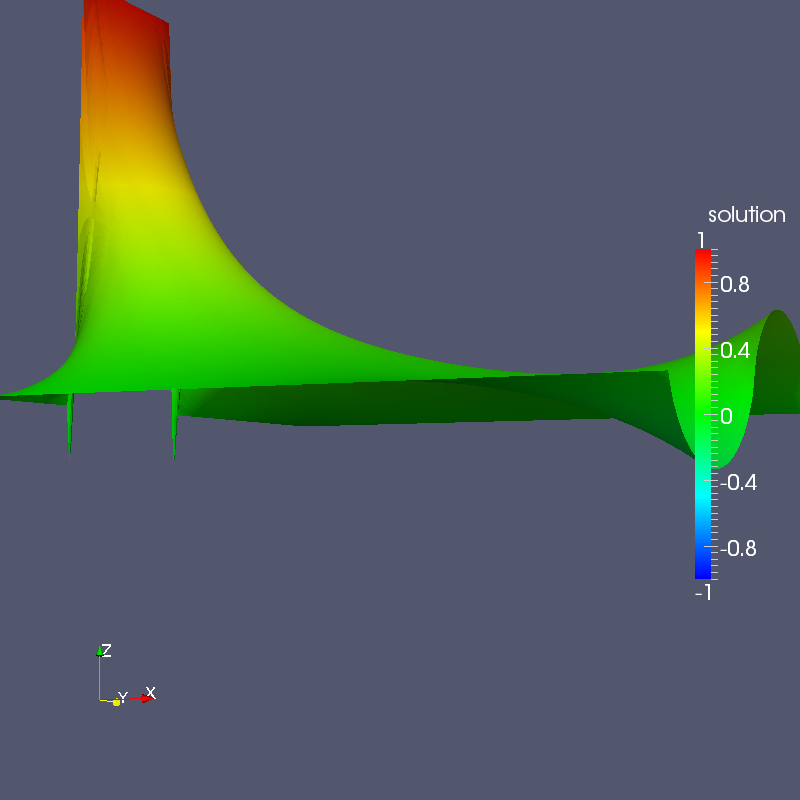
\includegraphics[width=0.65\textwidth]{./EPS/example03}}{example03.avi}
\end{center}
\end{frame}

\cleardoublepage

